\documentclass[11pt]{article}
\usepackage{amsmath}
\usepackage{amssymb}
\usepackage{relsize}
\usepackage{graphicx}

\begin{document}


Homework 1.4.4 Vector Length(norm2)
\\
\\
Compute the lengths of the following vectors:
\\
\\
(a)
$
\begin{bmatrix}
{0}\\
{0}\\
{0}\\
\end{bmatrix}$
\\
\\
Ans: 0
\\
\\
(b)
$
\begin{bmatrix}
{1/2}\\
{1/2}\\
{1/2}\\
{1/2}\\
\end{bmatrix}$
\\
\\
Ans: 1
\\
\\
(c)
$
\begin{bmatrix}
{1}\\
{-2}\\
{2}\\
\end{bmatrix}$
\\
\\
Ans: 3
\\
\\
(d)
$
\begin{bmatrix}
{0}\\
{0}\\
{1}\\
{0}\\
{0}\\
{0}\\
\end{bmatrix}$
\\
\\
Ans: 1
\\
\\
Homework 1.4.4.2
\\
\\
For $x$ $\in$ $\mathbb{R}^n$,
\\
\\
$\parallel$ $x$ $\parallel_{2}$ $<$ 0
\\
\\
NEVER
\\
\\
\\
\\
\\
\\
Homework 1.4.4.3
\\
\\
If $x$ is a unit vector then $x$ is a unit basis vector.
\\
\\
FALSE
\\
\\
Homework 1.4.4.4
\\
\\
If $x$ is a unit basis vector then $x$ is a unit vector.
\\
\\
TRUE
\\
\\
\newpage
Homework 1.4.4.5
\\
\\
If $x$ and $y$ are perpendicular (orthogonal) then $x^{T}$ $y$ = 0
\\
\\
\\
\begin{figure}
  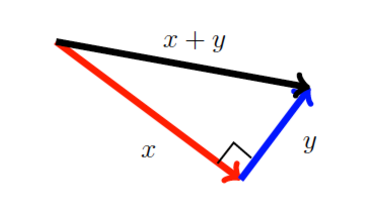
\includegraphics[width=\linewidth]{HW_1.png}
  \caption{Fig. 1.4.4.5}
  \label{Fig.1.4.4.5}
\end{figure}
\\
\\
\newpage
Homework 1.4.4.6
\\
\\
Let $x$,$y$ $\in$ $\mathbb{R}^n$ be nonzero vectors and let the angle between them
equal $\theta$. Then 
\\
\\
$cos$ $\theta$ = 
\\
\\
$\frac{x^{T}y}{\parallel x \parallel_{2} \parallel y \parallel_{2}}$
\\
\\
TRUE
\\
\\
Hint: Consider the picture and the "Law of Cosines"
\\
\\
\begin{figure}
  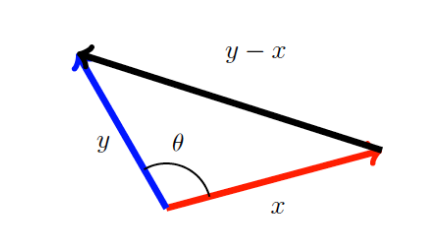
\includegraphics[width=\linewidth]{HW_2.png}
  \caption{Fig. 1.4.4.6}
  \label{Fig.1.4.4.6}
\end{figure}
\\
\\
\newpage
Homework 1.4.4.7
\\
\\
Let $x$,$y$ $\in$ $\mathbb{R}^n$ be nonzero vectors. Then $x^{T}$ $y$ = 0 if and only if $x$ and $y$ are orthogonal(perpendicular).
\\
\\
TRUE
\\
\\
Homework 1.4.4.8
\\
\\
What is the approximate cost of computing the length of a vector (if computed by a dot product)?
\\
\\
How many memops?
\\
\\
(a)n
\\
\\
How many flops?
\\
\\
(c)2n

\end{document}